\section{Problem Formulation}
Let $\mathcal{S}=\{\mathcal{V},\mathcal{E}\}$ be a source surface consisting of sample points $\mathcal{V}=\{\mathbf{v}_1, \mathbf{v}_2, \ldots, \mathbf{v}_n \in \mathbb{R}^3\}$ connected by a set of edges $\mathcal{E}$. Let $\mathcal{T}$ be a target surface with sample points $\mathcal{U}=\{\mathbf{u}_1, \mathbf{u}_2, \ldots, \mathbf{u}_m \in \mathbb{R}^3 \}$.
We seek to apply affine transformations to the source points $\mathcal{V}$ to align them with the target surface.
In this paper, we adopt the embedded deformation approach proposed in~\cite{sumner2007embedded} to model the transformations. Specifically, we construct a \emph{deformation graph} $\mathcal{G}$ with its vertices $\mathcal{V}_{\mathcal{G}} = \{\mathbf{p}_1,\ldots,\mathbf{p}_r\}$ being a subset of the source points $\mathcal{V}$, and with its edges $\mathcal{E}_{\mathcal{G}}$ connecting vertices that are nearby on the target surface.
On each deformation graph vertex $\mathbf{p}_j$ we define an affine transformation represented with a transformation matrix $\mathbf{A}_j \in \mathbb{R}^{3 \times 3}$ and a displacement vector $\mathbf{t}_j \in \mathbb{R}^3$. Each vertex $\mathbf{p}_j$ influences a localized region that contains any source point $\mathbf{v}_i$ whose geodesic distance $D(\mathbf{v}_i, \mathbf{p}_j)$ to $\mathbf{p}_j$ on the source surface is smaller than a user-specified radius $R$. If $\mathbf{p}_j$ influences a source point $\mathbf{v}_i$, the affine transformation $(\mathbf{A}_j, \mathbf{t}_j)$ associated with $\mathbf{p}_j$ induces a transformed position $\mathbf{A}_j(\mathbf{v}_i-\mathbf{p}_j)+\mathbf{p}_j + \mathbf{t}_j$ for $\mathbf{v}_i$.
Then the final transformed position $\newpos{\mathbf{v}}_i$ for $\mathbf{v}_i$ is a convex combination of all positions induced by the vertices in graph $\mathcal{G}$~\cite{li2009robust}:
\begin{equation}
\label{eq:sample_represent}
\newpos{\mathbf{v}}_i =  \sum_{\mathbf{p}_j \in \mathcal{I}(\mathbf{v}_i)} {w}_{ij} \cdot \left(\mathbf{A}_j(\mathbf{v}_i-\mathbf{p}_j)+\mathbf{p}_j + \mathbf{t}_j\right),
\end{equation}
where $\mathcal{I}(\mathbf{v}_i) = \{\mathbf{p}_j \mid D(\mathbf{v}_i, \mathbf{p}_j)<R \}$ denotes the set of vertices that influence $\mathbf{v}_i$, and ${w}_{ij}$ is a distance-dependent normalized weight:
\[
    {w}_{ij} = \frac{\left( 1 - {D^2(\mathbf{v}_i, \mathbf{p}_j)}/{R^2}\right)^3}
    {\sum_{\mathbf{p}_k \in \mathcal{I}(\mathbf{v}_i)} \left( 1 - {D^2(\mathbf{v}_i, \mathbf{p}_k)}/{R^2}\right)^3}.
\]
Compared to formulations that attach a different transformation to each source point such as~\cite{li2018robust}, a major benefit of using the deformation graph is that the deformation of the target surface can be defined with a much smaller number of variables, enabling more efficient optimization.

In the following, we first present an optimization formulation to determine the affine transformations associated with the deformation graph, and then explain how to construct the deformation graph. For the ease of presentation, we use $\mathbf{X}_j$ to denote the affine transformation $(\mathbf{A}_j, \mathbf{t}_j)$ at vertex $\mathbf{p}_j$, whereas $\mathbf{X}$ denotes the set of all transformations.


\subsection{Optimization Formulation}
\label{seq:model}

For robust alignment between the source and the target surfaces, we determine the affine transformations $\mathbf{X}$ via the following optimization:
\begin{equation}
\min_{\mathbf{X}}~ E_{\text{align}}(\mathbf{X}) + \alpha E_{\text{reg}}(\mathbf{X}) + \beta E_{\text{rot}}(\mathbf{X}).
\label{eq:model}
\end{equation}
Here the terms $E_{\text{align}}$, $E_{\text{smooth}}$, and $E_{\text{rot}}$ measures the alignment error, the regularization of transformations across the surface, and the deviation between the transformation matrices and rotation matrices, respectively. $\alpha$ and $\beta$ are positive weights that control the tradeoff between these terms. The definition for each term is explained in the following.



\paragraph{Alignment Term.}
For each transformed source point $\newpos{\mathbf{v}}_i$, we can find the closest target point $\mathbf{u}_{\rho(i)} \in \mathcal{U}$. The alignment term should penalize the deviation between $\newpos{\mathbf{v}}_i$ and $\mathbf{u}_{\rho(i)}$.
A simple approach is to define it as the sum of squared distances between all such pairs of points. This is indeed the alignment error metric used in the classical ICP algorithm~\cite{BeslM92} for rigid registration~\cite{Mitra2004}. On the other hand, such $\ell_2$-norm of pointwise distance can lead to erroneous alignment on real-world data, where the two surfaces might only overlap partially and their point positions might be noisy. This is because partial overlaps and noisy data can induce large distance from some source points to their corresponding target points under the ground-truth alignment, which would be prohibited by the $\ell_2$-norm minimization.

Some previous work, such as the Sparse ICP algorithm from~\cite{Bouaziz2013-SparseICP}, adopts the $\ell_p$-norm $(0 < p < 1)$ as the error metric. It is less sensitive to noises and partial overlaps, since $\ell_p$-norm minimization allows for large distances at some points. However, numerical minimization of the $\ell_p$-norm can be much more expensive than the $\ell_2$-norm. For example, the problem is solved in~\cite{Bouaziz2013-SparseICP} with an iterative algorithm that alternately updates the point correspondence and the transformation which is similar with classical ICP. However, its transformation update has to be done with an inner ADMM solver which is much slower than the closed-form update in classical ICP, and also lack convergence guarantee due to the non-convexity of the problem.

Inspired by the recent work from~\cite{ham2015robust} on robust image filtering and~\cite{zhang2018static} on robust mesh filtering, we adopt the following robust metric for the alignment error:
\begin{equation}
E_{\text{align}}(\mathbf{X}) = \sum_{i=1}^{n} \psi_{\nua}(\|\newpos{\mathbf{v}}_i -\mathbf{u}_{\rho(i)}\|),
\label{eq:Ealign}
\end{equation}
where $\psi_{\nua}(\cdot)$ is the Welsch's function~\cite{holland1977robust} (see Fig.~\ref{fig:welsch} left):
\[
    \psi_{\nua}(x)=1-\exp \left(-\frac{x^{2}}{2 \nua^{2}}\right),
\]
and $\nua > 0$ is a user-specified parameter.
$\psi_{\nua}$ is monotonically increasing on $[0, +\infty)$, thus $\psi_{\nua}(\|\newpos{\mathbf{v}}_i -\mathbf{u}_{\rho(i)}\|)$ penalizes the deviation between $\newpos{\mathbf{v}}_i$ and $\mathbf{u}_{\rho(i)}$. On the other hand, as $\psi_{\nua} \leq 1$, the deviation only induces a bounded influence on the metric $E_{\text{align}}$. Moreover, if $\nua \to 0$, then $E_{\text{align}}$ approaches the $\ell_0$-norm of the pointwise distance from the source points to their closest points on the target surface. Therefore, this error metric is insensitive to noisy data and partial overlaps.


\begin{figure}[!t]
	\centering
	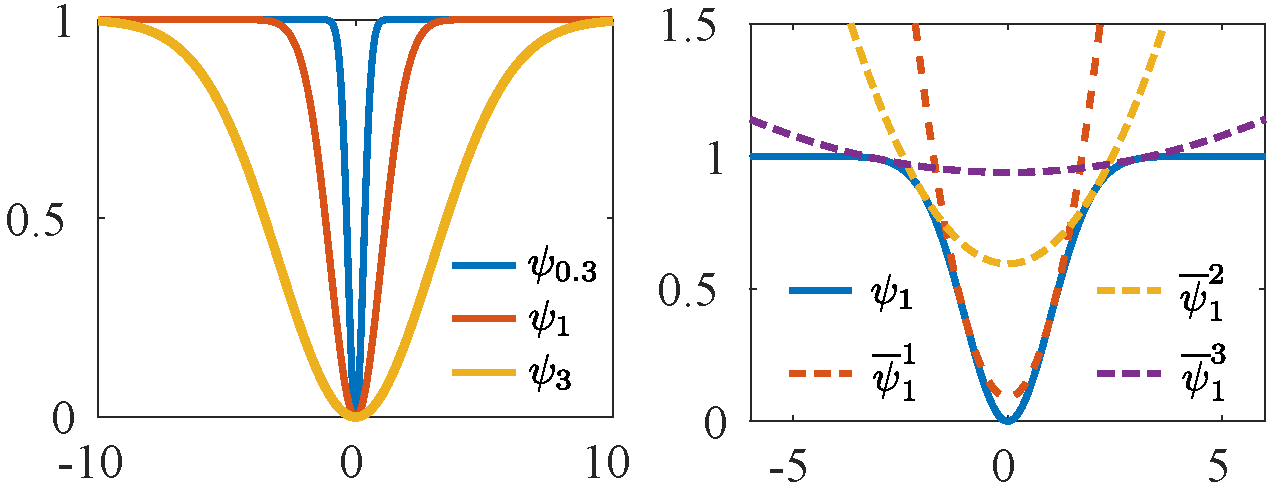
\includegraphics[width=1\columnwidth]{Figs/welsch_sur.pdf}
	\caption{Left: the Welsch's function with different $\nu$ values. Right: different surrogate functions for the Welsch's function with $\nu=1$.}
	\label{fig:welsch}
\end{figure}

\paragraph{Regularization Term.}
Ideally, the transformation induced by two neighboring vertices $\mathbf{p}_i, \mathbf{p}_j$ of the deformation graph should be consistent on their overlapping influenced regions. In~\cite{sumner2007embedded}, such consistency is measured at $\mathbf{p}_i$ using the difference of deformation induced by the transformation $\mathbf{X}_i$ at $\mathbf{p}_i$ and the transformation $\mathbf{X}_j$ at  $\mathbf{p}_j$:
\begin{equation}
    \mathbf{D}_{ij} = \mathbf{A}_j (\mathbf{p}_i - \mathbf{p}_j) + \mathbf{p}_j + \mathbf{t}_j - (\mathbf{p}_i + \mathbf{t}_i).
    \label{eq:Dij}
\end{equation}
Ideally, $\mathbf{D}_{ij}$ should be small across the deformation graph. On the other hand, in some cases the optimal deformation may induce large values of $\mathbf{D}_{ij}$ in some regions, such as the joints of a human body. To reduce the magnitudes of $\mathbf{D}_{ij}$ across the graph while allowing for large magnitudes in some regions, we define the regularization term using the Welsch's function on $\|\mathbf{D}_{ij}\|$:
\begin{equation}
    E_{\text{reg}}(\mathbf{X}) = \sum_{i=1}^r
    \sum_{\mathbf{p}_{j} \in \mathcal{N}(\mathbf{p}_{i})} \psi_{\nur}(\|\mathbf{D}_{ij}\|),
    \label{eq:Ereg}
\end{equation}
where $r$ is the number of nodes in $\mathcal{G}$, $\nur > 0$ is a user-specified parameter, and $\mathcal{N}(\mathbf{p}_{i})$ denotes the set of neighboring vertices for $\mathbf{p}_{i}$ in $\mathcal{G}$.

\paragraph{Rotation Matrix Term.} To preserve rigidity on local surface regions during registration, we would like each transformation $\mathbf{X}_i$ to be as close to a rigid transformation as possible. We measure this property using the deviation between the transformation matrix $\mathbf{A}_i$ and its closest projection onto the rotation matrix group $\SOG = \{\mathbf{R} \in \mathbb{R}^{3 \times 3} \mid \mathbf{R}^T \mathbf{R} = \mathbf{I}, \det(\mathbf{R}) > 0\}$, and define $E_{\text{rot}}$ as
\begin{equation}
E_{\text{rot}}(\mathbf{X}) = \sum_{i=1}^r\|\mathbf{A}_i - \proj\nolimits_{\SOG}(\mathbf{A}_i)\|_F^2,
\label{eq:rigid}
\end{equation}
where $\proj{}$ is the projection operator, and $\|\cdot\|_F$ is the Frobenius norm. 

\subsection{Construction of Deformation Graph}
To construct the deformation graph $\mathcal{G}$, we first extract its vertices $\mathcal{V}_{\mathcal{G}}$ by iteratively adding source points as follows. $\mathcal{V}_{\mathcal{G}}$ is initialized as empty. Then we perform PCA on all source points, and sort them based on their projections onto the axis with the largest eigenvalue of the covariance matrix. According to the sorted order, we go through each source point $\mathbf{v}_i$, and add it to $\mathcal{V}_{\mathcal{G}}$ if $\mathcal{V}_{\mathcal{G}}$ is empty or the shortest geodesic distance from $\mathbf{v}_i$ to the points in $\mathcal{V}_{\mathcal{G}}$ is no smaller than the radius parameter $R$. After determining the vertex set $\mathcal{V}_{\mathcal{G}}$, we construct the edge set $\mathcal{E}_{\mathcal{G}}$ by connecting any two vertices whose geodesic distance is smaller than $R$. We compute the geodesic distance using the fast marching method~\cite{kimmel1998computing}. $R$ is set to $5\overline{l}$ by default, where $\overline{l}$ is the average edge length on the source surface. Compared with alternative sampling strategies such as the farthest point sampling method~\cite{moenning2003fast}, our approach results in fewer sample points for the same radius parameter, which reduces the computational cost while achieving similar accuracy. A comparison example is provided in the supplementary material.


\section{Numerical Algorithm}
The target function $E$ for the optimization problem~\eqref{eq:model} is non-linear and non-convex.
Thanks to the use of the Welsch's function, it can be solved efficiently using the MM algorithm~\cite{Lange2004}. Specifically, given the variable values $\mathbf{X}^{(k)}$ in the current iteration, the MM algorithm constructs a surrogate function $\surrog{E}^{\mathbf{X}^{(k)}}$ for the target function $E$ such that
\begin{equation}
\label{eq:SurrogateE}
\begin{aligned}
\surrog{E}^{\mathbf{X}^{(k)}}(\mathbf{X}^{(k)}) & = E(\mathbf{X}^{(k)}),\\
\surrog{E}^{\mathbf{X}^{(k)}}(\mathbf{X}) &\geq E(\mathbf{X}), \quad \forall \mathbf{X} \neq \mathbf{X}^{(k)}.
\end{aligned}
\end{equation}
Then the variables are updated by minimizing the surrogate function
\begin{equation}
    \mathbf{X}^{(k+1)} = \argmin_{\mathbf{X}} \surrog{E}^{\mathbf{X}^{(k)}}(\mathbf{X}).
\end{equation}
In this way, each iteration is guaranteed to decrease the target function, and the iterations are guaranteed to converge to a local minimum regardless of the initialization~\cite{Lange2004}. In comparison, existing solvers for minimizing the non-convex $\ell_p$-norm such as ADMM~\cite{Bouaziz2013-SparseICP} or iteratively reweighted least squares~\cite{Daubechies2010} either lack convergence guarantee or rely on strong assumptions for convergence.  In the following, we explain the construction of the surrogate function, and present a numerical algorithm for its minimization in each iteration.

\subsection{Surrogate Function}
\label{sec:surrogate}
To construct the surrogate function $\surrog{E}^{\mathbf{X}^{(k)}}$, we note that there is a convex quadratic surrogate function for the Welsch's function $\psi_{\nu}$ at $y$~\cite{ham2015robust} (see Fig.~\ref{fig:welsch} right):
\[
    \surrog{\psi}_{\nu}^y (x) = \psi_{\nu}(y) + \left(\frac{1 - \psi_{\nu}(y)}{ 2 \nu^{2}}\right)\left(x^{2}-y^{2}\right).
\]
This function bounds the Welsch's function from above, and the two function graphs touch at $x = y$.
Applying this surrogate to all relevant terms, we obtain a surrogate function for ${E}_{\textrm{reg}}$ at $\mathbf{X}^{(k)}$. Moreover, we can ignore all constant terms as they do not affect the minimum, resulting in the following convex quadratic function
\begin{equation}
    \surrog{E}_{\textrm{reg}}^{\mathbf{X}^{(k)}}
    = \frac{1}{2 \nur^2} \sum_{i=1}^{r} \sum_{\mathbf{p}_{j} \in \mathcal{N}(\mathbf{p}_{i})} \exp\Big(-\frac{\|\mathbf{D}_{ij}^{(k)}\|^2}{2 \nur^2}\Big) \|\mathbf{D}_{ij}\|^2,
    \label{eq:RegSurrogate}
\end{equation}
where $\mathbf{D}_{ij}^{(k)}$ is evaluated using Eq.~\eqref{eq:Dij} at $\mathbf{X}^{(k)}$. Similarly, we can obtain the following function as a surrogate for ${E}_{\textrm{align}}$ at $\mathbf{X}^{(k)}$ up to a constant:
\begin{equation}
    \frac{1}{2 \nua^2} \sum_{i=1}^{n} \exp\Big(-\frac{\|\newpos{\mathbf{v}}_i^{(k)} -\mathbf{u}_{\rho(i)}^{(k)}\|^2}{2 \nua^2}\Big) \|\newpos{\mathbf{v}}_i -\mathbf{u}_{\rho(i)}\|^2,
    \label{eq:NaiveSurrogate}
\end{equation}
where $\newpos{\mathbf{v}}_i^{(k)}$ is the transformed position of $\mathbf{v}_i$ according to $\mathbf{X}^{(k)}$, and $\mathbf{u}_{\rho(i)}^{(k)}$ is the closest target point for $\newpos{\mathbf{v}}_i^{(k)}$. Eq.~\eqref{eq:NaiveSurrogate} is not a quadratic function of $\mathbf{X}$, as $\mathbf{u}_{\rho(i)}$ depends non-linearly on $\mathbf{X}$. To obtain a more simple form, we note that the term $\|\newpos{\mathbf{v}}_i -\mathbf{u}_{\rho(i)}\|^2$ has a quadratic surrogate function $\|\newpos{\mathbf{v}}_i -\mathbf{u}_{\rho(i)}^{(k)}\|^2$ at $\mathbf{X}^{(k)}$. Applying it to Eq.~\eqref{eq:NaiveSurrogate}, we obtain the following convex quadratic surrogate function for ${E}_{\textrm{align}}$  at $\mathbf{X}^{(k)}$ up to a constant:
\begin{equation}
\surrog{E}_{\textrm{align}}^{\mathbf{X}^{(k)}} = \frac{1}{2 \nua^2} \sum_{i=1}^{n} \exp\Big(-\frac{\|\newpos{\mathbf{v}}_i^{(k)} -\mathbf{u}_{\rho(i)}^{(k)}\|^2}{2 \nua^2}\Big) \|\newpos{\mathbf{v}}_i -\mathbf{u}_{\rho(i)}^{(k)}\|^2.
\label{eq:AlignSurrogate}
\end{equation}
Replacing ${E}_{\textrm{align}}$ and ${E}_{\textrm{reg}}$ in the target function with their surrogates, we arrive at the following MM iteration scheme:
\begin{equation}
    \mathbf{X}^{(k+1)} = \min_{\mathbf{X}} \surrog{E}^{\mathbf{X}^{(k)}} (\mathbf{X}),
    \label{eq:MMIeration}
\end{equation}
where
$\surrog{E}^{\mathbf{X}^{(k)}} = \surrog{E}_{\text{align}}^{\mathbf{X}^{(k)}} + \alpha \surrog{E}_{\text{reg}}^{\mathbf{X}^{(k)}} + \beta E_{\text{rot}}$.

\subsection{Numerical Minimization}

The target function $\surrog{E}^{\mathbf{X}^{(k)}}$ in Eq.~\eqref{eq:MMIeration} still contains a non-linear term $E_{\text{rot}}$, as the projection onto the rotation matrix group depends non-linearly on $\mathbf{A}_i$. On the other hand, as explained later, the special structure of $E_{\text{rot}}$ leads to a  simple form of its gradient, allowing us to evaluate the gradient of $\surrog{E}^{\mathbf{X}^{(k)}}$ efficiently. Therefore, we solve the sub-problem~\eqref{eq:MMIeration} using an L-BFGS solver for fast convergence. In each iteration, L-BFGS utilizes the gradients of $\surrog{E}^{\mathbf{X}^{(k)}}$ at the latest $m+1$ iterates $\mathbf{X}_{(j)}, \mathbf{X}_{(j-1)}, \ldots, \mathbf{X}_{(j-m)}$ to implicitly approximate its inverse Hessian and derive a descent direction $\mathbf{d}_{(j)}$, followed by a line search along $\mathbf{d}_{(j)}$ for a new iterate $\mathbf{X}_{(j+1)}$ with sufficient decrease of the target function~\cite{Nocedal2006}.
In the following, we present the details of the solver.

\paragraph{Gradient Computation.}
For the function $E_{\text{rot}}$ defined in Eq.~\eqref{eq:rigid}, each term $\|\mathbf{A}_i - \proj\nolimits_{\SOG}(\mathbf{A}_i)\|_F^2$ is the squared Euclidean distance from the matrix $\mathbf{A}_i$ to the manifold ${\SOG}$ of rotation matrices. Even though $\proj\nolimits_{\SOG}(\mathbf{A}_i)$ depends non-linearly on $\mathbf{A}_i$,  it can be shown that the squared distance has a simple form of gradient~\cite{Gomes2003}:
\[
    \frac{\partial \| \mathbf{A}_i - \proj\nolimits_{\SOG}(\mathbf{A}_i) \|^2}{\partial \mathbf{A}_i} = 2 \left(\mathbf{A}_i - \proj\nolimits_{\SOG}(\mathbf{A}_i)\right).
\]
Thus we can write the gradient of  $E_{\text{rot}}$ as:
\[
    \frac{\partial E_{\text{rot}}}{\partial \mathbf{A}_i} =  2 \left(\mathbf{A}_i - \proj\nolimits_{\SOG}(\mathbf{A}_i)\right),
    \quad
    \frac{\partial E_{\text{rot}}}{\partial \mathbf{t}_i} = \mathbf{0}.
\]
Since $\surrog{E}_{\text{align}}^{\mathbf{X}^{(k)}}$ and $\surrog{E}_{\text{reg}}^{\mathbf{X}^{(k)}}$ are quadratic functions, their gradients have simple linear forms. To facilitate presentation, we first rewrite the functions in matrix forms. In the following, we assume all 3D vectors are $3 \times 1$ matrices. The transformation at $\mathbf{p}_i$ is represented as $\mathbf{X}_i = [\mathbf{A}_i, \mathbf{t}_i]^T \in \mathbb{R}^{4 \times 3}$, and $\mathbf{X} = [ \mathbf{X}_1^T, \ldots, \mathbf{X}_r^T  ]^T \in \mathbb{R}^{4r \times 3}$. Then we have
\begin{equation}
     \surrog{E}_{\text{align}}^{\mathbf{X}^{(k)}}=\|\mathbf{W}_a (\mathbf{F}\mathbf{X}+\mathbf{P}-\mathbf{U})\|_F^2,
    \label{eq:alignMatrixForm}
\end{equation}
where $\mathbf{W}_a = \text{diag}(\sqrt{w_1^a},...,\sqrt{w_n^a}) \in \mathbb{R}^{n \times n}$ with
$
w_i^a = \frac{1}{2 \nua^2}  \exp\Big(-\frac{\|\newpos{\mathbf{v}}_i^{(k)} -\mathbf{u}_{\rho(i)}^{(k)}\|^2}{2 \nua^2}\Big)
$,
$\mathbf{F}$ is a block matrix  $\{\mathbf{F}_{ij}\}_{1 \leq i \leq n \atop 1 \leq j \leq r} \in \mathbb{R}^{n \times 4r}$ with
\[
\mathbf{F}_{ij}
    = \left\{
    \begin{array}{ll}
    w_{ij} \cdot [ \mathbf{v}_i^T - \mathbf{p}_j^T, 1 ] & \textrm{if}~\mathbf{p}_j \in \mathcal{I}(\mathbf{v}_i)\\
    \mathbf{0} & \textrm{otherwise}
    \end{array}
    \right.,
\]
and
$
    \mathbf{P}= \left[\sum_{\mathbf{p}_j \in \mathcal{I}(\mathbf{v}_i)} \mathbf{p}_j, \ldots, \sum_{\mathbf{p}_j \in \mathcal{I}(\mathbf{v}_n)} \mathbf{p}_j\right]^T \in \mathbb{R}^{n \times 3}
$,
$\mathbf{U}  = \left[ \mathbf{u}_{\rho(1)}^{(k)},..., \mathbf{u}_{\rho(n)}^{(k)}\right]^T \in \mathbb{R}^{n \times 3}.
$
Similarly, we have
\begin{equation}
\surrog{E}_{\text{reg}}^{\mathbf{X}^{(k)}} = \|\mathbf{W}_r(\mathbf{B} \mathbf{X} -\mathbf{Y})\|_F^2,
\label{eq:regMatrixForm}
\end{equation}
where the matrices $\mathbf{B} \in \mathbb{R}^{2 |\mathcal{E}_{\mathcal{G}}| \times 4 r}$ and $\mathbf{Y} \in \mathbb{R}^{2 |\mathcal{E}_{\mathcal{G}}| \times 3}$ encode the computation of a term $\mathbf{D}_{ij}$ in each row, and the diagonal matrix $\mathbf{W}_r$ stores the weight $\sqrt{\frac{1}{2 \nur^2}\exp\Big(-\frac{\|\mathbf{D}_{ij}^{(k)}\|^2}{2 \nur^2}\Big)}$ at the corresponding row.
In the row corresponding to $\mathbf{D}_{ij}$, the elements in $\mathbf{Y}$ are $[\mathbf{p}_j^T - \mathbf{p}_i^T]$, whereas the elements in $\mathbf{B}$ for $\mathbf{X}_i$ and $\mathbf{X}_j$ are $[\mathbf{p}_i^T - \mathbf{p}_j^T, 1]$ and $[0, 0, 0, 1]$, respectively.
We can further write the gradient of $E_{\text{rot}}$ in matrix form as
\[
    \frac{\partial E_{\text{rot}}}{\partial \mathbf{X}}
    = 2 (\mathbf{J} \mathbf{X} - \mathbf{Z}),
\]
where $\mathbf{Z} = [ \proj_{\mathcal{R}}(\mathbf{A}_1), \mathbf{0}, \ldots, \proj_{\mathcal{R}}(\mathbf{A}_r), \mathbf{0} ]^T \in \mathbb{R}^{4r \times 3}$, and $\mathbf{J} = \textrm{diag} (1, 1, 1, 0, 1, 1, 1, 0, \ldots, 1, 1, 1, 0) \in \mathbb{R}^{4r \times 4r}$.
We can then derive the gradient function of $\surrog{E}^{\mathbf{X}^{(k)}}$ as
\begin{equation}
\begin{aligned}
    \mathbf{G}(\mathbf{X})
     =~&2 [\mathbf{F}^T \mathbf{W}_a^2 (\mathbf{F}\mathbf{X}+\mathbf{P}-\mathbf{U}) \\
     &+
     \alpha \mathbf{B}^T \mathbf{W}_r^2(\mathbf{B} \mathbf{X} -\mathbf{Y})
        +
     \beta (\mathbf{J} \mathbf{X} - \mathbf{Z})].
\end{aligned}
\label{eq:Gradient}
\end{equation}


\begin{algorithm}[t!]
	%\LinesNumbered
	\label{Alg:TwoLoopRecursion}
	\caption{Two-loop recursion for computing descent direction $\mathbf{d}_{(j)}$}
	$\mathbf{Q} = - \mathbf{G}(\mathbf{X}_{(j)})$\;
	\For{$i = j-1, \ldots, j- m$}{
		$\mathbf{S}_i = \mathbf{X}_{i+1} - \mathbf{X}_i$;~
		$\mathbf{T}_i = \mathbf{G}(\mathbf{X}_{i+1}) - \mathbf{G}(\mathbf{X}_i)$\;
		$\rho_i = \Tr(\mathbf{T}_i^T \mathbf{S}_i)$\;
		$\xi_i = \Tr(\mathbf{S}_i^T \mathbf{Q}) / \rho_i$\;
		$\mathbf{Q} = \mathbf{Q} - \xi_i\mathbf{T}_i $\;
		
	}
	$\mathbf{R} = \mathbf{H}_0^{-1} \mathbf{Q}$\;
	\For{$i = j-m, \ldots, j- 1$}{
		$\eta = \Tr(\mathbf{T}_i^T \mathbf{R}) / \rho_i $\;
		$\mathbf{R} = \mathbf{R} + \mathbf{S}_i(\xi_i - \eta)$\;
	}
	$\mathbf{d}_{(j)} = \mathbf{R}$\;
\end{algorithm}


\paragraph{Computing $\mathbf{d}_{(j)}$ and $\mathbf{X}_{(j+1)}$.}
We adopt the L-BFGS implementation from~\cite{liu2017quasi} to utilize the special structure of $\surrog{E}^{\mathbf{X}^{(k)}}$.
Specifically, given an initial approximation $\mathbf{H}_{0}$ for the Hessian of $\surrog{E}^{\mathbf{X}^{(k)}}$ at $\mathbf{X}_{(j)}$,
we compute the descent direction $\mathbf{d}_{(j)}$ using a two-loop recursion explained in~\cite{liu2017quasi} (see Algorithm~\ref{Alg:TwoLoopRecursion}).
Following~\cite{liu2017quasi}, we derive $\mathbf{H}_{0}$ by assuming a fixed projection $\proj_{\mathcal{R}}(\mathbf{A}_i)$ for the term $E_{\text{rot}}$, resulting in the following approximation:
\begin{equation}
    \mathbf{H}_0 = 2 (\mathbf{F}^T \mathbf{W}_a^2 \mathbf{F}
    + \alpha \mathbf{B}^T \mathbf{W}_r^2\mathbf{B}
    +  \beta \mathbf{J}).
    \label{eq:InitialHessian}
\end{equation}
The new iterate $\mathbf{X}_{(j+1)}$ is then computed as
\[
    \mathbf{X}_{(j+1)} = \mathbf{X}_{(j)} + \lambda \mathbf{d}_{(j)},
\]
using a line search to determine the step size $\lambda > 0$ that achieve sufficient decrease of $\surrog{E}^{\mathbf{X}^{(k)}}$:
\begin{equation}
    \surrog{E}^{\mathbf{X}^{(k)}}(\mathbf{X}_{(j+1)})
    \leq
    \surrog{E}^{\mathbf{X}^{(k)}}(\mathbf{X}_{(j)}) +
    \gamma \lambda \Tr(\left(\mathbf{G}(\mathbf{X}_{(j)})\right)^T \mathbf{d}_{(j)}),
    \label{eq:SufficientDecrease}
\end{equation}
with $\gamma  \in (0, 1)$.
The iterative L-BFGS solver is terminated if $\surrog{E}^{\mathbf{X}^{(k)}}(\mathbf{X}_{(j)}) - \surrog{E}^{\mathbf{X}^{(k)}}(\mathbf{X}_{(j+1)}) < \epsilon_1$ where $\epsilon_1$ is a user-specified threshold. And the outer MM iteration is terminated if $\max_i\|\newpos{\mathbf{v}}^{(k+1)}_i - \newpos{\mathbf{v}}^{(k)}_i\| < \epsilon_2$ with a user-specified threshold $\epsilon_2$ or the number of outer iterations reaches a threshold $I_{\max}$.
In all experiments, we set $m = 5$, $\gamma = 0.3$, $\epsilon_1 = 10^{-3}$, $\epsilon_2 = 10^{-3}$, and $I_{\max} = 100$.

The matrix $\mathbf{H}_0$ is sparse symmetric positive definite and remains unchanged in each iteration of an L-BFGS solver. To solve the linear equation $\mathbf{R} = \mathbf{H}_0^{-1} \mathbf{Q}$ efficiently in the two-loop recursion, we compute a sparse Cholesky factorization for $\mathbf{H}_0$ at the beginning of an L-BFGS run, and reuse it in each iteration to solve the linear system with different right-hand-sides. In addition, the columns of the right-hand-side matrix $\mathbf{Q}$ are independent, thus we solve them in parallel. Moreover, although the matrix $\mathbf{H}_0$ may change between different L-BFGS runs, its sparsity pattern remains the same. Therefore, we pre-compute a symbolic factorization of $\mathbf{H}_0$ and only perform numerical factorization subsequently.

\paragraph{Choosing $\nua$ and $\nur$.}
To achieve robust registration, the values of $\nua$ and $\nur$ play an important role. Each of them acts as the standard deviation parameter for the Gaussian weight in the surrogate function~\eqref{eq:RegSurrogate} or \eqref{eq:AlignSurrogate}. The Gaussian weight becomes effectively zero for error terms whose current magnitude is much larger than the standard deviation. Both $\nua$ and $\nur$ need to be sufficiently small at the final stage of the solver, to exclude the influence of large error terms that arise from partial overlaps etc. On the other hand, at the initial stage of the solver, their values need to be larger in order to accommodate more error terms and achieve coarse alignment. Therefore, we initialize the variables $\mathbf{X}$ with a rigid transformation (see Sec.~\ref{sec:Results} for details), and solve the problem~\eqref{eq:model} with relatively large values $\nua = \nua^{\max}$ and $\nur = \nur^{\max}$. The solution is then used as initial variable values to re-solve the problem~\eqref{eq:model} with the values of $\nua$ and $\nur$ decreased by half. We repeat this process until the value of $\nua$ reaches a lower bound $\nua^{\min}$, and take the final solution as the registration result. Algorithm~\ref{Alg:total-alg} summarizes our overall registration algorithm with gradually decreased values of $\nua$ and $\nur$.
By default, we set $\nur^{\max} = 40 \overline{l}$, $\nua^{\max} = 10 \overline{d}$ and $\nua^{\min} = 0.5 \overline{l}$, where $\overline{d}$ is the medium distance from source points to their corresponding target points under the initial rigid transformation, and $\overline{l}$ is the average edge length on the source surface. In the supplementary material, we compare our strategy of gradually decreasing $\nua$ and $\nur$ with registration using fixed $\nua$ and $\nur$, which shows that our strategy achieves a more accurate result.


\begin{algorithm}[!t]
\LinesNumbered
\label{Alg:total-alg}
\caption{Non-rigid registration}
$\nu_a=\nu_a^{\max};~~\nu_r = \nu_r^{\max}$\;
%;~~$k=0$
\While{TRUE}{
	%$k_{\max} = k + I_{\max}$\;
    $k=0$\;
    \Repeat{$\max_i\|\newpos{\mathbf{v}}^{(k+1)}_i - \newpos{\mathbf{v}}^{(k)}_i\| < \epsilon_2$ OR $k = I_{\max}$}{
        Find correspoding point $\mathbf{u}_{\rho(i)}^{(k)}$ for each $\newpos{\mathbf{v}}_i^{(k)}$\;
        Update weight matrices $\mathbf{W}_{a}$ and $\mathbf{W}_r$\;
        $j = -1$;~~ $\mathbf{X}_{(0)} = \mathbf{X}^{(k)}$\;
         \Repeat{$\surrog{E}^{\mathbf{X}^{(k)}}(\mathbf{X}_{(j)}) - \surrog{E}^{\mathbf{X}^{(k)}}(\mathbf{X}_{(j+1)}) < \epsilon_1$}{
        $j = j+1$\;
        Compute gradient $\mathbf{G}(\mathbf{X}_{(j)})$ with~\eqref{eq:Gradient}\;
        Compute direction $\mathbf{d}_{(j)}$ with Alg.~\ref{Alg:TwoLoopRecursion}\;
        Perform line search for $\mathbf{X}_{(j+1)}$ that satisfies condition~\eqref{eq:SufficientDecrease}\;
        }
        $\mathbf{X}^{(k+1)}=\mathbf{X}_{(j+1)}$\;
        $k = k+1$\;
    }
    \If{$\nu_a = \nu_a^{\min}$}
    {
        return $\mathbf{X}^{(k+1)}$\;
    }
    $\nu_a =\max(0.5 \cdot \nu_a, \nu_a^{\min})$;~~
    $\nu_r = 0.5 \cdot \nu_r$\;
}
\end{algorithm}

\paragraph{Setting of $\alpha$ and $\beta$.} To account for the number of terms in each component of the target function in Eq.~\eqref{eq:model}, we set the weights as $\alpha=k_\alpha (|\mathcal{V}|/|\mathcal{E}_{\mathcal{G}}|)$ and $\beta= k_\beta (|\mathcal{V}|/|\mathcal{V}_{\mathcal{G}}|) $, with  $k_\alpha = k_\beta = 1$ by default. We decrease the values of $k_\alpha$ and $k_\beta$ on problem instances with reliable initialization to achieve better alignment, and increase their values on problem instances with less reliable initialization to avoid converging to an undesirable local minimum. Moreover, the value of $k_\alpha$ can be increased for smoother deformation of the source surface, or decreased for faster convergence.

